\chapter{Background}

\epigraph{A honeypot is a security resource whose value lies in being probed, attacked, or compromised.}{\textit{Lance Spitzner}}

Using honeypots in a cloud environment merge two varying principals together.
This chapter introduces the fundamental knowledge that is needed to comprehend the upcoming experiments.
If the reader has a profound understanding of cloud computing, honeypots, and virtualization he can skip this chapter.

\section{Virtualization}

Virtualization, often referred to \ac{vm}, is defined by \citet{kreuter2004} as \enquote{an abstraction layer or environment between hardware component and the end-user}.
A \ac{vm} runs on top of the \ac{os} core components.
Through an abstraction layer, the virtual machine is connected with the real machine by hypervisors or \ac{vmm}.
Hypervisors can use real machine hardware components, but also support virtual machine operating systems and configurations.
Both are similar to emulators, that are defined by \citet{lichstei1969} as \enquote{process whereby one computer is set up to permit the execution of programs written for another computer}.
This allows to manage multiple \ac{vm} with real machine resources.
There are three different types of virtualization,
\begin{enumerate*}[label=(\roman*)]
    \item software virtual machines,
    \item hardware virtual machines, and
    \item virtual OS/containers
\end{enumerate*}.
Software virtual machine's manage interactions between the host operating system and guest operating system.
Hardware virtual machine's offers direct and fast access to the underlying resources.
It uses hypervisors, modified code, or APIs.
Lastly, virtual OS/container partitions the host operating system into containers or zones.
\cite{daniels2009}

\section{Cloud Computing}
\label{sec:cloud-computing}

Cloud Computing has become a very popular keyword these days. 
It has been used by various large companies such as Google and Amazon.
However, the term \enquote{cloud computing} dates back to the late 1996, when a small group of technology executives of Compaq Computer framed new business ideas around the Internet.\cite{regalado2020}
Starting from 2007 cloud computing evolved into a serious competitor and outnumbered the keywords \enquote{virtualization}, and \enquote{grid computing} as reported by Google trends \cite{Wang2010}.
Shortly, various cloud providers become publicly available, each with their own strengths and weaknesses.
For example IBM's Cloud\footnote{\url{https://www.ibm.com/cloud}}, Amazon Web Services\footnote{\url{https://aws.amazon.com/}}, and Google Cloud\footnote{\url{https://cloud.google.com/}}.
Why are clouds so attractive in practice?

\begin{itemize}
    \item It offers major advantages in terms of cost and reliability.
    When demand is needed, consumers do not have to invest in hardware when launching new services.
    Pay-as-you-go allows flexibility.
    \item Consumers can easily scale with demand.
    When more computational resources are required due to more requests, scaling up instances in conjunction with a suited price model are straightforward.
    \item Geographically distributed capabilities supply the need for world-wide scattered services.
\end{itemize}

\subsection{Definition of Cloud Computing}

With reference to the definition by Brian Hayes, cloud computing is \enquote{a shift in the geography of computation} \cite{hayes2008}.
Thus, computational workload is moved away from local instances towards services and datacenters that provide the user's needs\cite{Armbrust2010}.

The \ac{nist} defines cloud computing as \enquote{a model for enabling ubiquitous, convenient, on-demand network access to a shared pool of configurable computing resources (e.g., networks, servers, storage, applications, and services) that can be rapidly provisioned and released with minimal management effort or service provider interaction} \cite{Mell2011}.
\ac{nist} not only reflects the geographical shift of resources such as datacenters, but also mentions on-demand usage that contributes to a flexible resource management.
Moreover, \ac{nist} composes the term in five essential characteristics, three service models (see \autoref{subsec:cloud-service}), and four deployment models (see \autoref{subsec:cloud-deployment}) \cite{Mell2011}

\textit{On-demand-self-service} refers to the unilateral provision computing capabilities.
Consumers can acquire server time and network storage on demand without a human interaction.

\textit{Broad network access} characterizes the access of capabilities of the network through standard protocols such as \ac{http}.
Heterogeneous thin and thick client platforms should be supported.

\textit{Resource pooling} allows the provider's computing resources to be pooled across several consumers.
A multi-tanent model with different physical and virtual resources are assigned on demand.
Other aspects such as location are independent and cannot be controlled on a low-level by consumers.
Moreover, high-level access to specify continent, state, or datacenter can be available.

\textit{Rapid elasticity} offers consumers to extend and release capabilities easily.
Further automatization to quickly increase resources  when demand skyrockets significantly can be supported regardless limit and quantity at any time.

\textit{Measured service} handles resources in an automated and optimized manner.
It uses additional metering capabilities to trace storage, processing, bandwidth, and active user accounts.
This helps to monitor, and control resource usage. Thus, contributing to transparency between provider and consumer.

\subsection{Service models}
\label{subsec:cloud-service}

Service models are categorized by \ac{nist} into three basic models based on usage and abstraction level.
\autoref{fig:cloud-functionalities} shows the connection between each model whereas cloud resource are defined in \autoref{subsec:cloud-deployment}.
Due to the vast range of functionalities, \ac*{iaas} builds the foundation of service models.
Each model on top represents a user-friendly abstraction with derated capabilities.

\begin{figure}[ht]
    \centering
    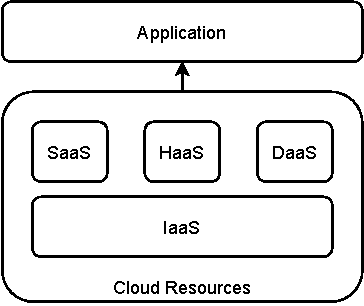
\includegraphics[width=0.4\textwidth]{figures/cloud-service-models.pdf}
    \caption[Abstract visualization of service models]{Abstract visualization of service models. The lowest level within the container \enquote{cloud resources} represents the depth of functionalities. Therefore, \ac{iaas} offers the most functionalities whereas the others have a user-friendly abstraction.}
    \label{fig:cloud-functionalities}
\end{figure}

\ac{saas} is a high-level abstraction to consumers. Controlling the underlying infrastructure is not supported.
Providers often use a multi-tenancy system architecture to organize each consumer's application in a separate environment.
It helps to employ scaling with respect to speed, security availability, disaster recovery, and maintenance.
Main objective of \ac{saas} is to host consumer's software or application that can be accessed over the Internet using either a thin or rich client. \cite{Dillon2010}
\enquote{Limited user-specific application configuration settings} can be made \cite{Mell2011}.

\ac{paas} pivots on the full \enquote{Software Lifecycle} of an application whereas \ac{saas} distinct on hosting complete applications.
\ac{paas} offers ongoing development and includes programming environment, tools, configuration management, and other services.
In addition, the underlying infrastructure is not managed by the consumer. \cite{Mell2011}

\ac{iaas} offers a low-level abstraction to consumers with the ability to run arbitrary software regardless of operating system or application.
In contrast to \ac{saas}, IT infrastructure capabilities (such as storage, networks) can be used.
It strongly depends on virtualization due to integration, or decomposition of physical resources. \cite{Mell2011}

\ac{daas} serves as a virtualized data storage service on demand. Motivations behind such services could be upfront costs of on-premise enterprise database systems. \cite{Dillon2010}
Mostly they require \enquote{dedicated server, software license, post-delivery services, and in-house IT maintenance} \cite{Dillon2010}
Whereas \ac{daas} costs solely what consumer's need.
When dealing with a tremendous amount of data, file systems and RDBMS often lack in performance.
\ac{daas} outruns such weak links by employing a table-style abstraction that can be scaled. \cite{Dillon2010}

\ac{haas} offers IT hardware, or datacenters to buy as a pay-as-you-go subscription service.
The term dates back to 2006 during a time when hardware virtualization became more powerful.
It is flexible, scalable and manageable. \cite{Wang2010}

\subsection{Deployment models}
\label{subsec:cloud-deployment}

Deployment models are categorized by \ac{nist} into four basic models.
Each differs in data privacy, location, and manageability \cite{Mell2011}.

Private clouds offer the highest level of control in regard of data privacy, and utilization. Mostly, such clouds are deployed within in a single organization, either managed by in-house teams or third party suppliers.
In addition, it can be on or off premise.
Within private clouds consumers have full control of their data.
Especially for European data privacy laws, it is not negligible when data is stored abroad and thus under law of foreign countries.
However, its popularity has not been diminished due to the immense cost of switching to public clouds. \cite{Dillon2010, Mell2011}

Community clouds can be seen as a conglomerate of multiple organizations that merge their infrastructure with respect to a commonly defined policy, terms, and condition beforehand. \cite{Mell2011}

Public clouds represent the most used deployment models.
In contrary, to private one, public clouds are fully owned by the service provider such as business, academics, or government organization.
Consumers do not know where their data is distributed.
In addition, contracts underlie custom policies. \cite{Mell2011}

Hybrid cloud is a mixture of two or more cloud infrastructures, such as private and public cloud.
However, each entity keeps its core element.
Hybrid clouds defines \enquote{standardized or proprietary technology to enables data and application portability}\cite{Mell2011}.

\section{Honeypots}

The term \enquote{honeypot} exists since more than a decade.
1997 was the first time that a free honeypot solution became public.
\ac{dtk}, developed by Fred Cohen, released the first honeypot solution.
However, the earliest drafts of honeypots are from 1990/91, and built the foundation for Fred Cohen's \ac*{dtk}.
Clifford Stoll's book \enquote{The Cuckoo's Egg}\cite{stroll2000}, and Bill Cheswick's whitepaper \enquote{An Evening With Berferd}\cite{Cheswick92} describe concepts that are considered nowadays as honeypots.\cite{Spitzner2003}
A honeypot itself is a security instrument that collects information on buzzing attacks.
It disguises itself as a system, or application with weak links, so that it gets exploited and gathers knowledge about the adversary.
In 2002 a Solaris honeypot helped to detect an unknown \verb|dtspcd| exploit.
Interestingly, a year before in 2001 the Coordination Center of \ac{cert}, \enquote{an expert group that handles computer security incidents}\cite{cert2021}, shared their concerns regarding the dtspcd.
Communities were aware that the service could be exploited to get access and remotely compromise any Unix system.
However, during this time such an exploit was not known, and experts did not expect any in the near future.
Gladly, early instances based on honeypot technologies could detect new exploits and avoid further incidents.
Such events lay emphasis on the importance of honeypots.

\subsection{Definition of a Honeypot}

A dozen of definitions for honeypots circulate through the web that causes confusion, and misunderstandings.
In general, the objective of a honeypot is to gather information about attacks, or attack patterns \cite{NawrockiWSKS2016}.
Thus, contributing as an additional source of security measure.
See \autoref{subsec:honeypot-security-concept} for a detailed view regarding honeypots in the security concept.
As \citet{Spitzner2003} has listed, most misleading definitions are: honeypot is a tool for deception, it is a weapon to lure adversaries, or a part of an intrusion detection system.
In order to get a basic understanding, we want to exhibit some key definitions.
\citet{Spitzner2003} defines honeypots as a \enquote{security resource whose value lies in being probed, attacked, or compromised}.
Independent of its source (e.g. server, application, or router), we expect that our instance is getting probed, attacked, and eventually exploited.
If a honeypot does not match this behaviour, it will not provide any value.
It is important to mention that honeypots do not have any production value, thus, any communication that is acquired is suspicious by nature \cite{Spitzner2003}.
In addition, \citet{Spitzner2003} points out that honeypots are not bounded to solve a single problem, hence, they function as a generic perimeter, and fit into different situation.
Such functions are attack detection, capturing automated attacks, or alert/warning generator.
\autoref{fig:honeypot-example} show an example how honeypots could be used in an IT infrastructure.

\begin{figure}[ht]
    \centering
    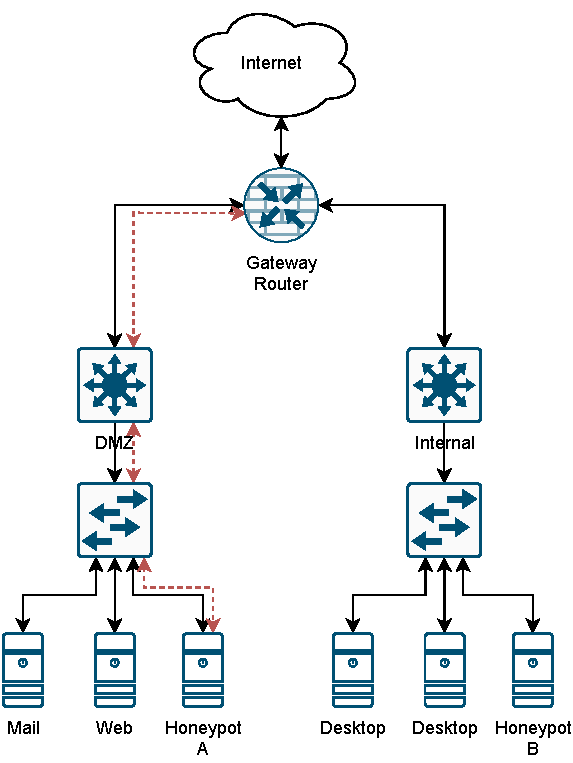
\includegraphics{figures/honeypot-example.pdf}
    \caption[Example of honeypots in a simplified network]{Example of honeypots in a simplified network (derived from \cite{Spitzner2003}). Each of the \ac{dmz}, and internal network are separated by a router and a Layer-3 switch. As derived from above, in each network a honeypot is available (honeypot A, B). The read path symbolizes the path of an attacker coming from the gateway router.}
    \label{fig:honeypot-example}
\end{figure}

In general, we differentiate two types of honeypots
\begin{enumerate*}[label=(\roman*)]
    \item Production honeypots
    \item Research honeypots
\end{enumerate*}.
This categorization has their origin from Mark Rosch developer of Snort during his work at GTE Internetworking.

Production honeypots are the common type of honeypots that people would think of.
The objective is to protect production environments, and to mitigate the risk of attacks.
Normally, production honeypots are easy to deploy within an organization.
Mostly, low-interaction honeypots are chosen due to a significant reduce in risk.
Thus, adversaries might not be able to exploit honeypots to attack other systems.
The downside of a low-interaction honeypot is a lack of information, for example standard information like the origin of attacks, or what exploits are used can be collected, whereas insides about communication of attackers, or deployment of such attacks are unlikely to obtain.
In contrast, research honeypots do fulfill this objective. \cite{Spitzner2003}

Research honeypots are used to learn more in detail about attacks.
The objective is to collect information about the clandestine organizations, new tools for attacks, or the origin of attacks.
Research honeypots are unlikely suitable for production environments due to a higher increase of risk.
Facing an increase in deployment complexity, and maintenance does not attract a production usage either. \cite{Spitzner2003}

It is worth to mention that there is no exact line between research or production honeypots.
Possible cases are honeypots that could function as either a production or a research honeypot.
Due to their dynamic range in which they are applicable it makes it hard to distinguish.

\citet{Provos2003} adds a differentiation for the virtual honeypot framework and splits it into the following types:

\begin{itemize}
    \item Physical honeypots are \enquote{real machines on the network with its own IP address} \cite{Provos2003}
    \item Virtual honeypots are \enquote{simulated by another machine that responds to network traffic sent to the virtual honeypot} \cite{Provos2003}
\end{itemize}

\subsection{Level of Interaction}
\label{subsec:interaction-honeypots}

When building and deploying a honeypot, the depth of information has to be defined beforehand.
Should it gather unauthorized activities, such as an \textsc{nmap} scan?
Do you want to learn about buzzing tools and tactics?
Each depth brings a different level of interaction because some information depends on more actions of adversaries.
Therefore, honeypots differ in level of interaction.

Low-interaction honeypots provide the lowest level of interaction between an attacker and a system.
Only a small set of services like SSH, Telnet, or FTP are supported which contributes to the deployment time.
In terms of risk, a low-interaction honeypot does not give access to the underlying \ac{os} which makes it safe to use in a production environment.
For example, using an SSH honeypot, such services are emulated, thus, attackers can attempt to log in by brute force or by guessing, and execute commands.
However, the adversary will never gain more access because it is not a real \ac{os}.
However, safety comes with the downside of less information.
Collection is limited for statistical purpose such as
\begin{enumerate*}[label=(\roman*)]
    \item time and data of attack
    \item source IP address and source port of the attack
    \item destination IP address and destination port of the attack
\end{enumerate*}.
Transactional information can not be collected. \cite{Spitzner2003}

A medium-interaction honeypot offers more sophisticated services with higher level of interaction.
It is capable to respond to certain activities.
For example, a Microsoft IIS Web server honeypot could be able to respond in a way that a worm is expecting it.
The worm would get emulated answers, and could be able to interact with it more in detail.
Thus, gathering more severe information about the attack, including privilege assessment, toolkit capturing, and command execution.
In comparison, medium-interaction honeypots allocate more time to install and configure.
Also, more security checks have to be performed due to a higher interaction level than low-interaction honeypots. \cite{Spitzner2003}

High-interaction honeypots represent a real \ac{os} to provide a full set of interactions to attackers.
They are so powerful because other production servers do not differ much to high-interaction honeypots.
They represent real systems in a controlled environment.
Obviously, the amount of information is tremendous. It helps to learn about
\begin{enumerate*}[label=(\roman*)]
    \item new tools
    \item finding new bugs in the \ac{os}
    \item the black hat community
\end{enumerate*}. However, the risk of such a honeypot is extremely high.
It needs severe deployment and maintenance processes, thus, it is time-consuming.

\subsection{Security concepts}
\label{subsec:honeypot-security-concept}

Security concepts are classified by \citet{Schneier2004} in prevention, detection, and reaction.
Prevention includes any process that
\begin{enumerate*}[label=(\roman*)]
    \item discourages intruders and
    \item hardens systems to avoid any kind of breaches
\end{enumerate*}.
Detection scrutinizes the identification of attacks that threatens the systems'
\begin{enumerate*}[label=(\roman*)]
    \item confidentiality
    \item integrity and
    \item availability
\end{enumerate*}.
Reaction treats the active part of the security concept.
When attacks are detected, in conducts reactive measures to remove the threat.
Each part is designed to be sophisticated so that all of them contribute to a secure environment. \cite{NawrockiWSKS2016}

Honeypots contribute to the security concept like firewalls, or \ac{ids}. Regarding prevention, honeypots add only a small value because security breaches cannot be identified.
Moreover, attackers would avoid wasting time on honeypots and go straight for production systems instead.

However, detection is one of the strengths of honeypots.
Attacks often vanish in the sheer quantity of production activities.
If any connection is obtained to a honeypot it is suspicious by nature.
In conjunction with an alerting tool, attacks can be detected.

Honeypots strongly supply reaction tools due to their clear data.
In production environments, finding attacks for further data analysis are not easy to grasp.
Often data submerge with other activities which complicates the process of reaction. \cite{NawrockiWSKS2016}
\citet{NawrockiWSKS2016} distinct honeypots from other objectives such as firewall, or log-monitoring.

\begin{table}[ht]
    \centering
    \caption[Distinction between security concepts]{Distinction between security concepts based on areas of operations (derived from \cite{NawrockiWSKS2016}).}
    \begin{tabular}{l|lll}
        \toprule
        \textbf{Objective}        & \textbf{Prevention} & \textbf{Detection} & \textbf{Reaction} \\ \hline
        Honeypot                  & +                   & ++                 & +++               \\
        Firewall                  & +++                 & ++                 & +                 \\
        Intrusion Detection Sys.  & +                   & +++                & +                 \\
        Intrusion Prevention Sys. & ++                  & +++                & ++                \\
        Anti-Virus                & ++                  & ++                 & ++                \\
        Log-Monitoring            & +                   & ++                 & +                 \\
        Cybersecurity Standard   & +++                 & +                  & +                 \\
        \bottomrule
    \end{tabular}
    \label{tab:honeypots-security-concepts}
\end{table}

\subsection{Value of Honeypots}

To assess the value of honeypots we want to take a closer look to their advantages and disadvantages.\cite{Mokube2007,Kaur2014,Spitzner2003}

\subsubsection{Advantages}

\begin{itemize}
    \item Data Value: Collected data is often immaculate and does not contain noise from other activities.
          Thus, reducing the total size of data, and speeding up the analyzation.
    \item Resources: Firewalls, and \ac{ids} are often overwhelmed by the gigabits of traffic, thus, dropping network packets for analyzation.
          This results in a far less effective detection for malicious network activities.
          However, honeypots are independent of resources because they only capture their activities at itself.
          Due to resource limitation, expensive hardware is not needed.
    \item Simplicity: A honeypot do not require any complex algorithms, or databases.
          A user should be able to quickly deploy it somewhere.
          Research honeypots might come with a certain increase of complexity. 
          However, if a honeypot is complex, it will lead to misconfigurations, breakdowns, and failures.
    \item Return on Investment: Capturing attacks immediately informs users that suspicious activities occur on the infrastructure.
          This helps to demonstrate their value, and contributes to new investment in other security measurements.
\end{itemize}

In addition, \citet{NawrockiWSKS2016} listed four more advantages of honeypots:

\begin{itemize}
    \item Independent of Workload: Honeypots only process traffic that is direct to them.
    \item Zero-Day-Exploit Detection: It helps to detect unknown strategies and zero-day-exploits.
    \item Flexibility: Well-adjusted honeypots for a variety of specific tasks are available.
    \item Reduced False Positives and Negatives: Any traffic or connection to a honeypot is suspicious.
          Client-honeypots verify such attacks based on system state changes.
          This results in either false positive, or false positive.
\end{itemize}

\subsubsection{Disadvantages}

\begin{itemize}
    \item Narrow Field of View: Only direct attacks on honeypots can be investigated whereas attacks on production system are not detected.
    \item Fingerprinting: A honeypot often has a certain fingerprint that can be identified by attackers.
          Especially commercial ones can be detected by their responses or behaviors.
    \item Risk to the Environment: Using honeypots in an environment always increase the risk.
          However, it depends on the level of interaction.
\end{itemize}

\subsection{Honeynets}

Instead of having single honeypots that can be attacked, a honeynet offers a complete network of standard production systems such as you would find in an organization.
Those systems are high-interaction honeypots, thus, allowing to fully interact with the \ac{os}, and applications.
Key idea is that an adversary can probe, attack, and exploit these systems so that we can derive interaction within this network.
It should be mentioned that a honeynet have to be protected by firewalls.
\autoref{fig:honeynet-example} represents such a honeynet within an organization.

\begin{figure}[ht]
    \centering
    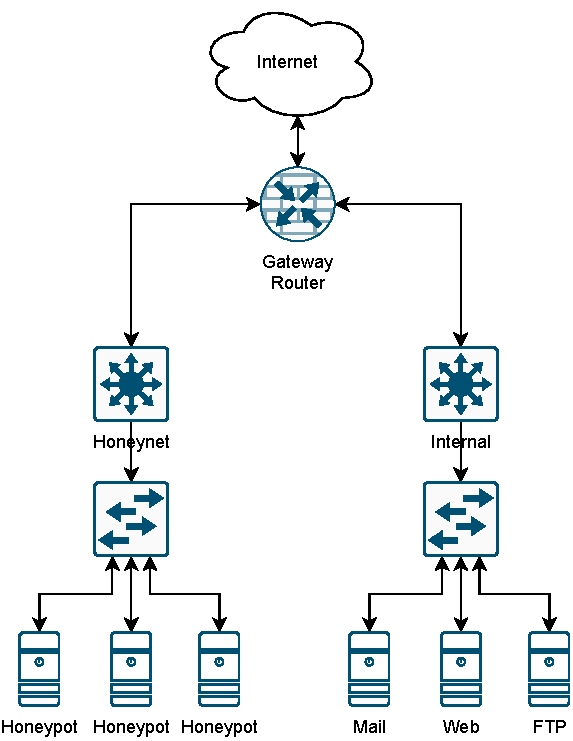
\includegraphics{figures/honeynet-example.pdf}
    \caption[Example of honeynets in a simplified network]{Example of honeynets in a simplified network (derived from \cite{Spitzner2003}). On the left, this network presents the honeynet consisting of several other honeypots. On the right the network presents an ordinary subnet consisting of mail, web, and FTP server.}
    \label{fig:honeynet-example}
\end{figure}

In comparison to a regular honeypot, the greatest value of honeynets is the usage of true production systems.
Black hats often do not know that they attack a honeynet, thus, adding value to prevention.
However, the downsides are high complexity and maintenance that is needed to keep a honeynet running. \cite{Spitzner2003}

\subsection{Legal Issues}

Considering questions related to legal issues of honeypots can easily exceed this thesis.
In this regard, we restrict the study to the country we reside in.
Thus, we are only concerned about the \ac{eu} regulations, EU directives, and international agreements.
Honeypots collect
\begin{enumerate*}[label=(\roman*)]
    \item content data that is used for communication, and
    \item transactional data that is used to establish the connection
\end{enumerate*}.
\citet{sokol2017} studied the legal conditions for data collection and data retention. They come to the conclusion that administrators of honeypots have a legal ground of legitimate interest to store and process personal data, such as IP addresses. Moreover, for production honeypots the legitimate interest is to secure services. Regarding the length of data retention, the principle of data minimization has to be considered which means there is no clear answer for it. Any published data of research honeypots needs to be anonymized.

\subsection{Related Work}

The Snort \cite{caswell2003} inline extension \textit{Bait'n'Switch} \cite{gonzalez2003} redirects attackers from production systems to honeypots.
Usually Snort drops malicious packets when they are detected, and creates a specific rule to block malicious activity from the source.
In contrast, \textit{Bait'n'Switch} does not create a rule to block more request, instead it redirects them to honeypots.
The attacker does not realize that all packets are rerouted, and that the original target has changed.
The \ac{ids} is bounded to its signature database and can only redirect known attacks. \cite{Diebold2005}

Whereas \textit{Bait'n'Switch} had to drop the first attack which leads to a suspicious behavior for attackers, the \textit{Intrusion Trap System} \cite{takemori2003} is capable of forwarding the first request.
Therefore, the first recognized attack by the \ac{ids} can be forwarded and answered by honeypots. \cite{Diebold2005}

The \textit{honeyd} \cite{Provos2003} extension \textit{Honeycomb} \cite{kreibich2004} enables automatically generates \textit{Snort} and \textit{Bro} \cite{paxson1999} signatures for all incoming traffic.
In addition, new signatures are created for similar patterns if they do not exist already, and updating of existing ones to improve their quality.
This is based on the incoming traffic, and the corresponding attack session.
Even mutations of attacks are considered.
It generates a more generic description for signatures in order to match the original attack, and the mutation.
It helps to keep the size of signatures small.
However, the downside of this extension is the missing verification of attacks.
Wrongly redirected traffic will not be proofed if an attack was successful even though a signature has been created. \cite{Diebold2005}
